\chapter{Crystallography and Point Defects}

\label{ch:crystallography}

\section{\zirconia\ phases}
{\setstretch{1.5}
\zirconia\ is unusual in exhibiting three commonly reported polytypes in its binary phase diagram. The temperature-pressure phase diagram of \zirconia\ as currently understood is shown in Figure \ref{figure:currentphasediagram}, with phase details collated in Table \ref{table:phases}. Each will now be described and contrasted.
}
%(see Figure \ref{figure:binary_phase_diagram})

\begin{figure}[htp] % Current phase diagram
\centering
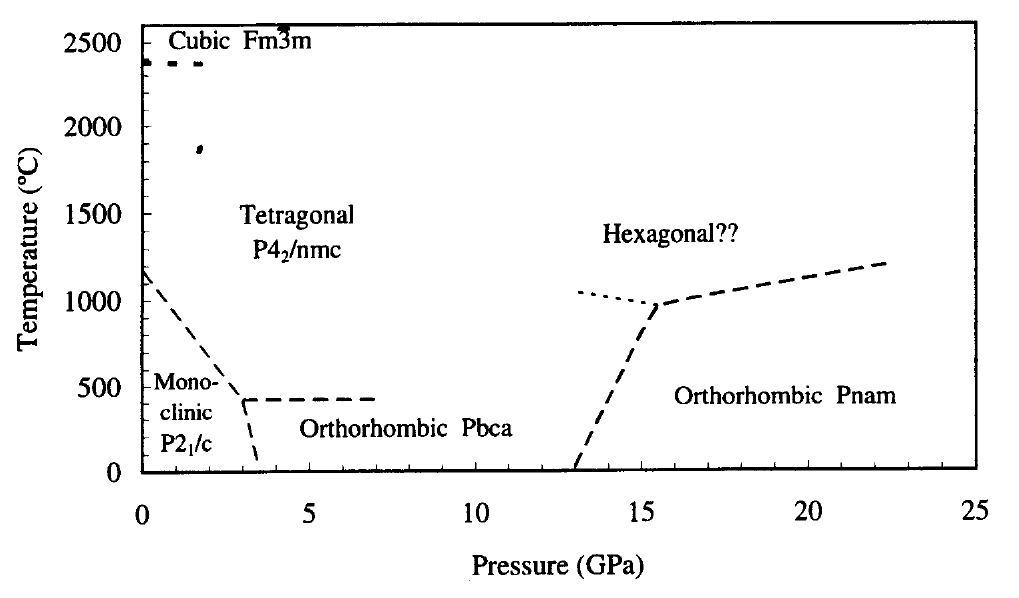
\includegraphics[height=7.7cm]{images/current_phase_diagram.png}
\caption[Temperature-pressure phase diagram of \zirconia .]{Temperature-pressure phase diagram of \zirconia . Taken from \cite{kisi1998crystal}.
\label{figure:currentphasediagram}}
\end{figure}

\begin{landscape}
\begin{center}
\begin{table}[htp]
\onehalfspacing
\centering
\caption[\zirconia\ phases and their details.]{\zirconia\ phases and their details. Adapted from \cite{kisi1998crystal}.}
\label{table:phases}
%\resizebox{\textwidth}{!}{%
\begin{tabular}{ccccccccccc}
\hline
\multirow{3}{*}{Phase} & \multirow{3}{*}{\begin{tabular}[c]{@{}c@{}}Stability\\ range\\ (K, GPa)\end{tabular}} & \multicolumn{4}{c}{\multirow{2}{*}{\begin{tabular}[c]{@{}c@{}}Cell parameters (\r{A})\\ (Extrapolated to room temperature)\end{tabular}}} & \multicolumn{4}{c}{\multirow{2}{*}{Atom positions}} & \multirow{3}{*}{\begin{tabular}[c]{@{}c@{}}Space\\ group\end{tabular}} \\
 &  & \multicolumn{4}{c}{} & \multicolumn{4}{c}{} &  \\ \cline{3-10}
 &  & $a$ & $b$ & $c$ & $\beta$ & Atom & $x$ & $y$ & $z$ &  \\ \hline
\multirow{2}{*}{Cubic \cite{terblanche1989thermal}} & \multirow{2}{*}{2377-2710 K} & \multirow{2}{*}{5.117} & \multirow{2}{*}{5.117} & \multirow{2}{*}{5.117} & \multirow{2}{*}{90} & Zr & 0 & 0 & 0 & \multirow{2}{*}{F$m\overline{3}m$} \\
 &  &  &  &  &  & O & 0.25 & 0.25 & 0.25 &  \\ \hline
\multirow{2}{*}{Tetragonal \cite{LANG1964}} & \multirow{2}{*}{1205-2377 K} & \multirow{2}{*}{5.074} & \multirow{2}{*}{5.074} & \multirow{2}{*}{5.188} & \multirow{2}{*}{90} & Zr & 0 & 0 & 0 & \multirow{2}{*}{P$4_{2}/nmc$} \\
 &  &  &  &  &  & O & 0.25 & 0.25 & 0.2044 &  \\ \hline
\multirow{3}{*}{Monoclinic \cite{Howard1988}} & \multirow{3}{*}{0-1205 K} & \multirow{3}{*}{5.1507} & \multirow{3}{*}{5.2028} & \multirow{3}{*}{5.3156} & \multirow{3}{*}{99.194} & Zr & 0.2754 & 0.0395 & 0.2083 & \multirow{3}{*}{P$2_{1}/c$} \\
 &  &  &  &  &  & O1 & 0.0700 & 0.3317 & 0.3477 &  \\
 &  &  &  &  &  & O2 & 0.4416 & 0.7569 & 0.4792 &  \\ \hline
\multirow{3}{*}{Ortho I \cite{ohtaka1990structural}} & \multirow{3}{*}{3.5-15 GPa} & \multirow{3}{*}{5.0431} & \multirow{3}{*}{5.2615} & \multirow{3}{*}{5.0910} & \multirow{3}{*}{90} & Zr & 0.2686 & 0.0332 & 0.2558 & \multirow{3}{*}{P$bca$} \\
 &  &  &  &  &  & O1 & 0.0822 & 0.3713 & 0.1310 &  \\
 &  &  &  &  &  & O2 & 0.5442 & 0.2447 & 0.0052 &  \\ \hline
\multirow{3}{*}{\begin{tabular}[c]{@{}c@{}}Ortho II \cite{Haines1995} \\ (cotunnite)\end{tabular}} & \multirow{3}{*}{\textgreater 15 GPa} & \multirow{3}{*}{5.593} & \multirow{3}{*}{6.484} & \multirow{3}{*}{3.333} & \multirow{3}{*}{90} & Zr & 0.256 & 0.110 & 0.25 & \multirow{3}{*}{P$nma$} \\
 &  &  &  &  &  & O1 & 0.356 & 0.422 & 0.25 &  \\
 &  &  &  &  &  & O2 & 0.022 & 0.331 & 0.75 &  \\ \hline
\multirow{3}{*}{Ortho (PSZ) \cite{kisi1989crystal}} & \multirow{3}{*}{0-500 K} & \multirow{3}{*}{5.068} & \multirow{3}{*}{5.260} & \multirow{3}{*}{5.077} & \multirow{3}{*}{90} & Zr & 0.267 & 0.030 & 0.250 & \multirow{3}{*}{P$bc2_{1}$} \\
 &  &  &  &  &  & O1 & 0.068 & 0.361 & 0.106 &  \\
 &  &  &  &  &  & O2 & 0.537 & 0.229 & 0 &  \\ \hline
\end{tabular}%
\end{table}
\end{center}
\end{landscape}

%Zirconia-based ceramics are used in a variety of technological and commercial applications, ranging from thermal barriercoatings on aircraft turbines to affordable diamond substitutes[167,168]. Recently, zirconia has received attention as an alternative dielectrics to silicon dioxide for memory and logic devices [169]. The versatility of zirconia originates entirely fromatomic or point defects in the crystal created by adding aliovalent oxides, e.g., MgO, La2O3, and Y2O3. The substitutionalcations or dopants that are charge balanced by the formation ofoxygen vacancies, and their mutual interactions, dramaticallyaffect the structural, thermal, mechanical, and electrical properties of modified or stabilized zirconia (SZ). These defects aresolely responsible for the high ionic conductivity of doped zirconia that underlies its use in oxygen sensors [170], and hightemperature fuel cells [171]. Zirconia is also used as a support material in heterogeneous catalysis [172].


\subsection{Monoclinic}

Below 1205 K at atmospheric pressure, \zirconia\ adopts a monoclinic Baddeleyite (P$2_{1}/c$) crystal structure. This is the ground state structure of \zirconia . In this phase, Zr ions have a sevenfold O coordination, down from eight in the higher temperature phases due to a single broken bond. A unit cell of monoclinic \zirconia\ is illustrated in Figure \ref{figure:coordination}. The dashed line (approximately 3.7\r{A} in length) shows the Zr-O bond which is broken when transitioning to monoclinic from the tetragonal phase. Zr-O bond lengths range from 2.05 to 2.31 \r{A}.

\begin{figure}[htp] % Mono coordination figure
\centering
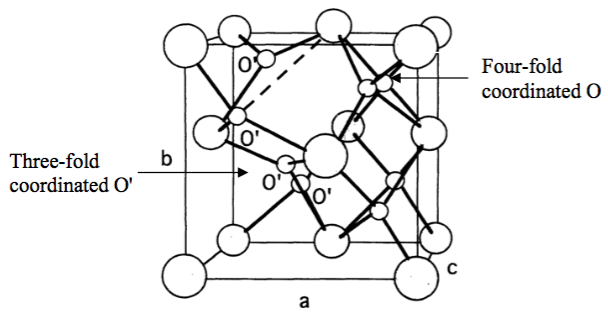
\includegraphics[height=7.5cm]{images/coordination.png}
\caption[A monoclinic zirconia unit cell indicating the two different oxygen bond coordinations. Small spheres represent oxygen ions while large spheres represent zirconium ions.]{A monoclinic zirconia unit cell indicating the two different oxygen bond coordinations. Small spheres represent oxygen ions while large spheres represent zirconium ions. Taken from \cite{Xia2010}.
\label{figure:coordination}}
\end{figure}

Monoclinic phase \zirconia\ also has two distinct oxygen ions in its primitive cell. To maintain the stoichiometry of 1:2 Zr to O, half of the oxygen ions exhibit threefold coordination with zirconium (in a planar configuration), while the other half have a fourfold coordination (tetrahedral configuration) with zirconium. Figure \ref{figure:monoschottky} shows the positions of these oxygen ions around a zirconium ion centre. The distortion from the oxygen rock salt sub-lattice can be seen, specifically in the case of the three coordinated oxygen ions. This is due to the zirconium ion being too small to hold 8 oxygen ions in an octahedral configuration, as in the fluorite crystal structure. As temperature is increased, so too are the interatomic distances. At the tetragonal temperature range, bonding between all 8 nearest neighbour oxygen and zirconium ions becomes energetically favourable and there is a transition to eightfold coordination.

\begin{figure}[htp] % Mono Zr centre
\centering
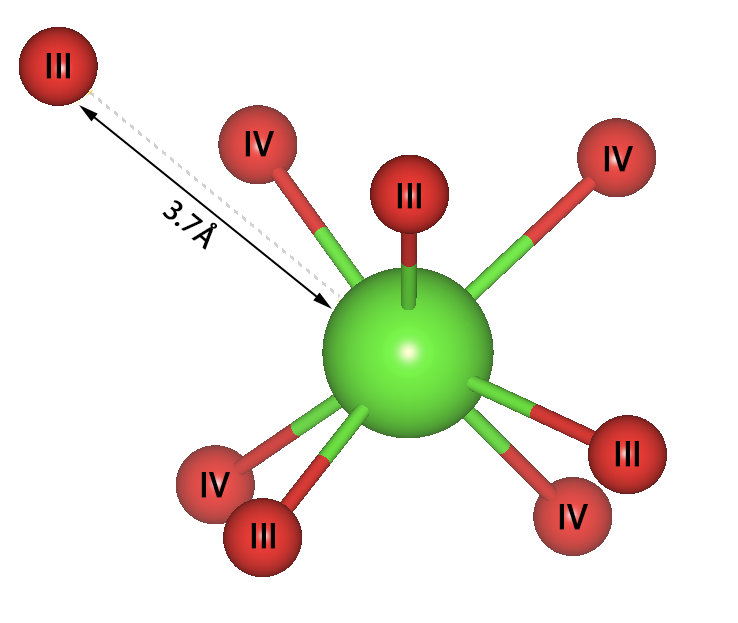
\includegraphics[height=8.5cm]{images/mono_zr_centre.png}
\caption{Zirconium centre unit cell in monoclinic \zirconia\ showing nearest oxygen atoms and their respective bond co-ordinations. Zirconium atoms are shown in green and oxygen atoms in red.}
\label{figure:monoschottky}
\end{figure}


The monoclinic-tetragonal phase transition occurs by a diffusionless martensitic transformation with a 9\textdegree\ shear \cite{Subbarao1974}. This is a fast transformation and is accompanied by a large volume change. Tetragonal phase \zirconia\ (density 6.10 g/cm$^{3}$) is around 4.6\% more dense than monoclinic \zirconia\ (density 5.83 g/cm$^{3}$) \cite{McCullough2002}, though the volume increase when cooling from tetragonal has been reported to be as high as 9\% \cite{Gupta1977}. This results in a kinetic barrier between the phases, and therefore the phase transition exhibits a hysteresis loop approximately 200 K wide when undergoing thermal cycling, as shown in Figure \ref{figure:hysteresis_monotet}.

\begin{figure}[htp] % Hysteresis
\centering
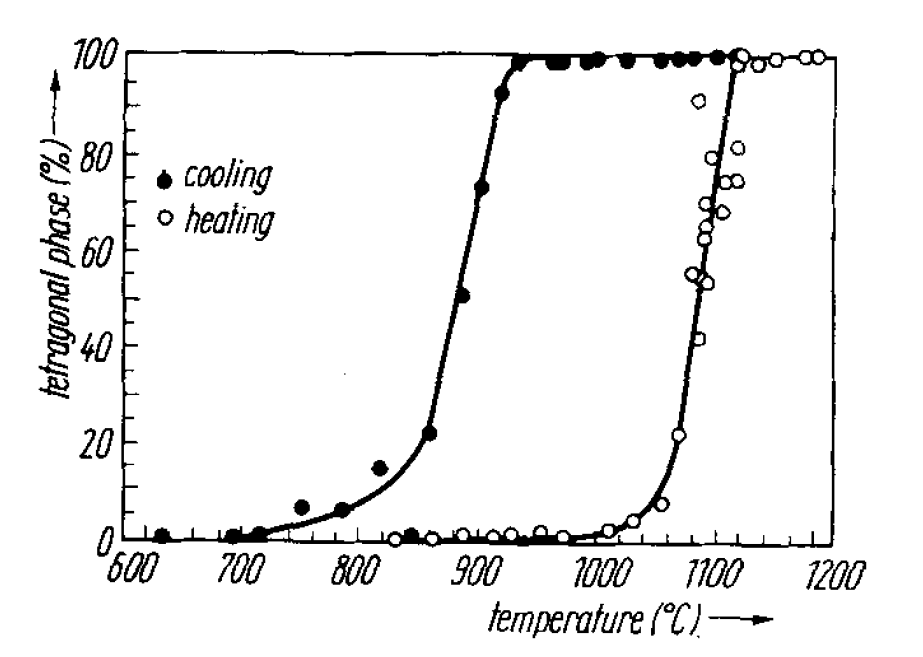
\includegraphics[width=12cm]{images/hysteresis_monotet.png}
\caption[Monoclinic-tetragonal phase transition in \zirconia\ as a function of temperature only.]{Monoclinic-tetragonal phase transition in \zirconia\ as a function of temperature only. Taken from \cite{WOLTEN1963}.}
\label{figure:hysteresis_monotet}
\end{figure}






%\begin{table}[htp]
%\centering
%\onehalfspacing
%\caption{\zirconia\ crystal structures and their stable temperatures at 1 atm \cite{Howard1988}.}
%\label{table:phases}
%\begin{tabular}{ccc}
%\hline
%{Crystal Structure} & {Space Group}    & {Temperature Range (K)} \\ \hline
%\multicolumn{1}{c}{Monoclinic} & \multicolumn{1}{c}{$P2_1/c$} & \multicolumn{1}{c}{$T$ \textless\ 1440}     \\
%\multicolumn{1}{c}{Tetragonal} & \multicolumn{1}{c}{$P4_2/nmc$} & \multicolumn{1}{c}{1440 \textless\ $T$ \textless\ 2640}        \\
%\multicolumn{1}{c}{Cubic} & \multicolumn{1}{c}{$Fm\overline{3}m$}     & \multicolumn{1}{c}{2640 \textless\ $T$ \textless\ 2950}      \\ \hline
%\end{tabular}
%\end{table}

\subsection{Tetragonal}

The tetragonal phase (space group P$4_{2}/nmc$) can be easily derived from the cubic phase by shifting alternating columns of oxygen ions slightly up or down the [001] direction. This change is so subtle that the two phases are almost identical when viewed in certain orientations. Figure \ref{figure:tetvscubic} shows a view of a  tetragonal phase unit cell down the [110] direction alongside a [100] view of a cubic phase unit cell. Going from the cubic to the tetragonal phase, the oxygen ions can clearly be seen to deviate from their equilibrium sites in the cubic sublattice. This is consistent with the interpretation that the ionic radius of Zr is slightly too small to maintain the cubic fluorite structure, which is therefore only seen at high temperatures (where thermal fluctuations mean the effective ionic radii are larger) or when under high compressive stress (where interatomic spacings are smaller).

\begin{figure}[htp]
\centering
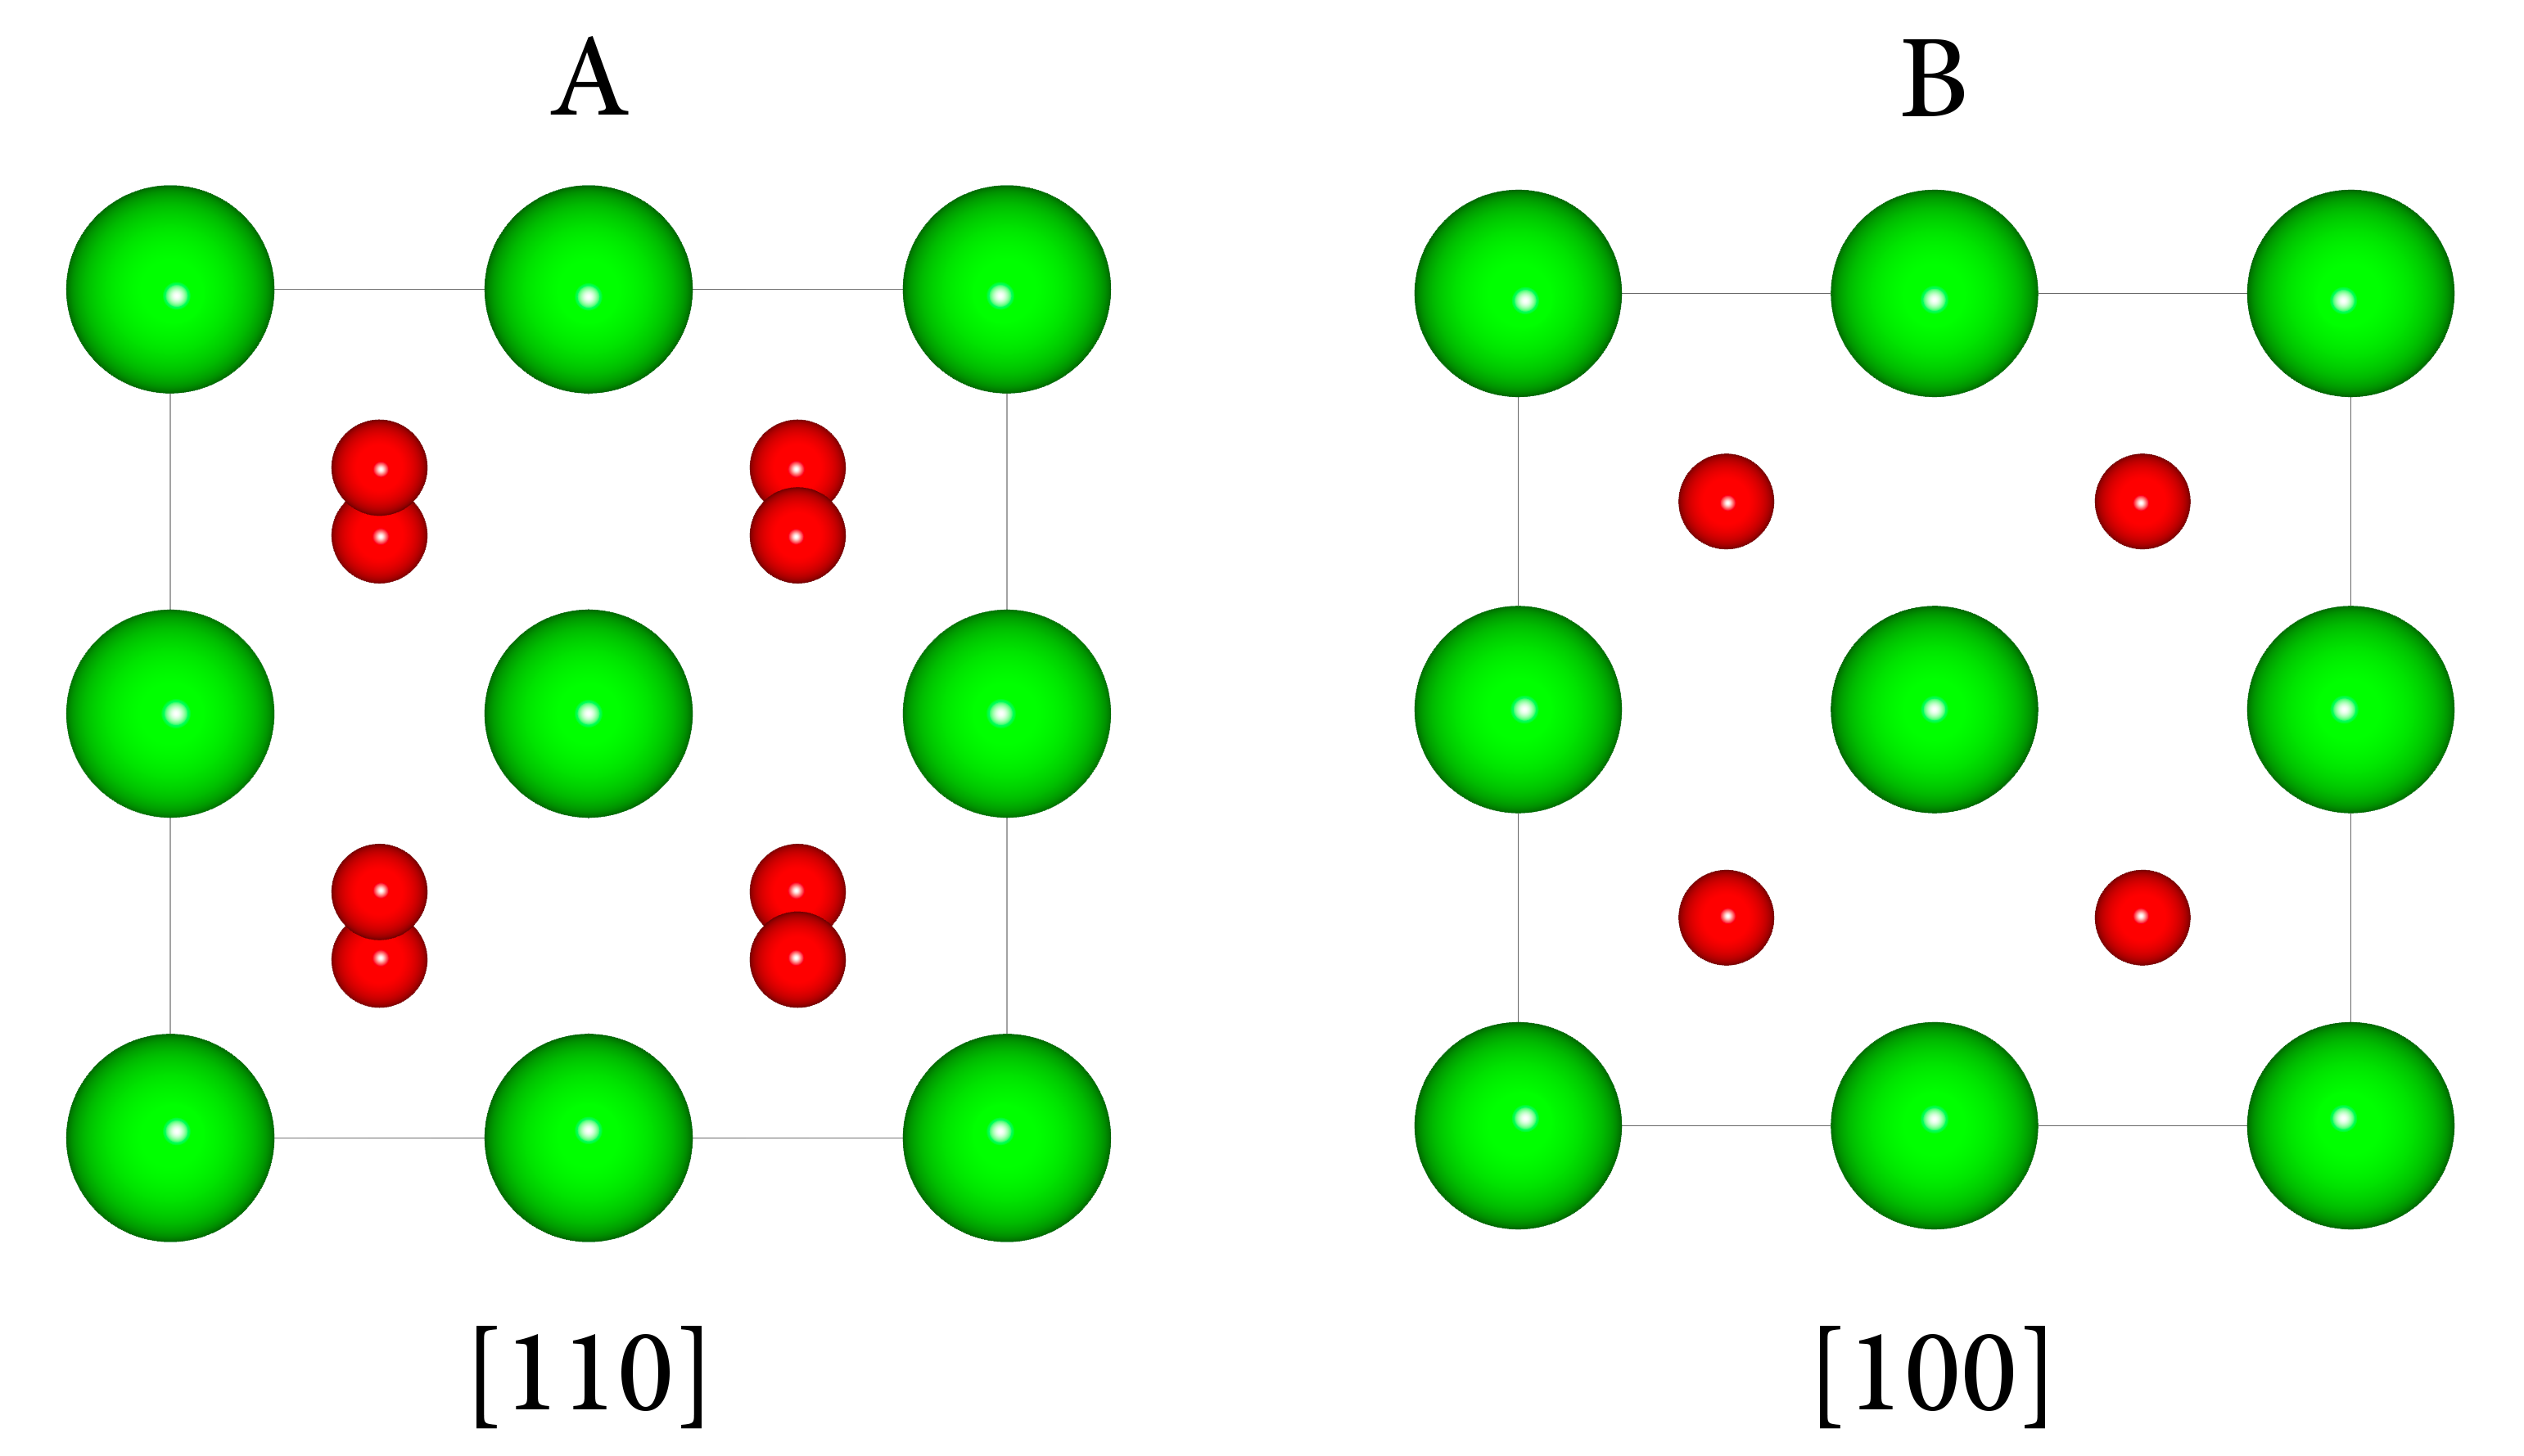
\includegraphics[width=14cm]{images/tet_vs_cubic.png}
\caption{\textbf{A}) Tetragonal \zirconia\ viewed along the [110] direction. \textbf{B}) Cubic \zirconia\ viewed along the [100] direction. Zirconium atoms are shown in green and oxygen atoms in red.}
\label{figure:tetvscubic}
\end{figure}

\subsubsection{Tetragonal phase stress stabilisation}

The pressure-temperature phase diagram of \zirconia\ (Figure \ref{fig:phasediagram}) shows how the monoclinic-tetragonal phase transition temperature is strongly dependent on pressure, with an almost linear reduction in transition temperature of 300\textdegree C GPa$^{-1}$. The phase diagram also shows the extent of the hysteresis effect in the monoclinic-tetragonal transition.

\begin{figure}[htp]
  \centering
      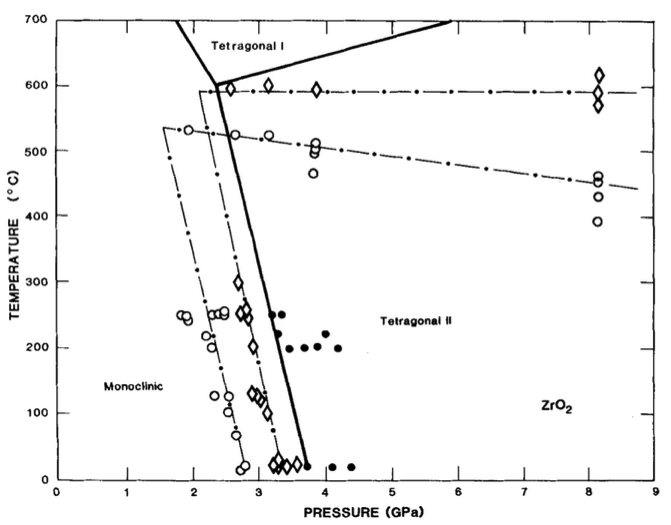
\includegraphics[width=13cm]{images/zirconiaphasediagram.png}
  \caption[Pressure-temperature phase diagram for \zirconia . Dash-dotted lines represent more recent data. Diamonds mark transition points during an increase in temperature of pressure, while open circles represent a decrease in pressure or temperature. Solid circles represent transition points for a fresh, single crystal sample.]{Pressure-temperature phase diagram for \zirconia . Dash-dotted lines represent more recent data. Diamonds mark transition points during an increase in temperature of pressure, while open circles represent a decrease in pressure or temperature. Solid circles represent transition points for a fresh, single crystal sample. Taken from \cite{block1985pressure}. \label{fig:phasediagram}}
\end{figure}

There is some degree of tetragonal phase autostabilisation during the oxidation process of zirconium. This is possible because of the resulting increase in volume when zirconium is oxidised. Zirconium has a Pilling-Bedworth ratio of 1.57, meaning that the oxide would occupy a volume 57\% larger than the metal if unconstrained \cite{cramer2003corrosion, Pilling1923}. In the case of zirconia, the oxide grows into the metal by dissolution of oxygen, generating large compressive stresses of up to 2 GPa \cite{Petigny2000, garzarolli1991oxide}. This is an important contribution to the stabilisation of the tetragonal phase because of the strong dependence on pressure, though this contribution alone may not be sufficient at PWR operating temperatures.

Stabilisation of the tetragonal phase at low temperatures is also dependent on grain size, which can be controlled during the cladding manufacturing process since the oxide inherits the grain size of the zirconium metal grains. Pure \zirconia\ exhibits a strong relationship between grain size and phase stability, where the tetragonal phase is only stable when grown from metal grains below a critical size of approximately 30 nm \cite{barberis1995zirconia}. This can be explained by increased dislocation interaction in smaller grains due to limited room for dislocation glide, as per the Hall-Petch relationship \cite{hall1951deformation, petch1953cleavage}. Grains of tetragonal \zirconia\ larger than this critical size are therefore likely to have tetragonal-stabilising dopant ions incorporated in the lattice.

\subsection{Cubic}

Cubic \zirconia\ (unit cell shown in Figure \ref{fig:cubic_unitcell}) adopts the cubic fluorite (space group F$m\overline{3}m$) crystal structure, consisting of zirconium ions in a face-centred cubic configuration with a rock salt oxygen sub-lattice occupying the tetrahedral sites.

\begin{figure}[htp]
  \centering
      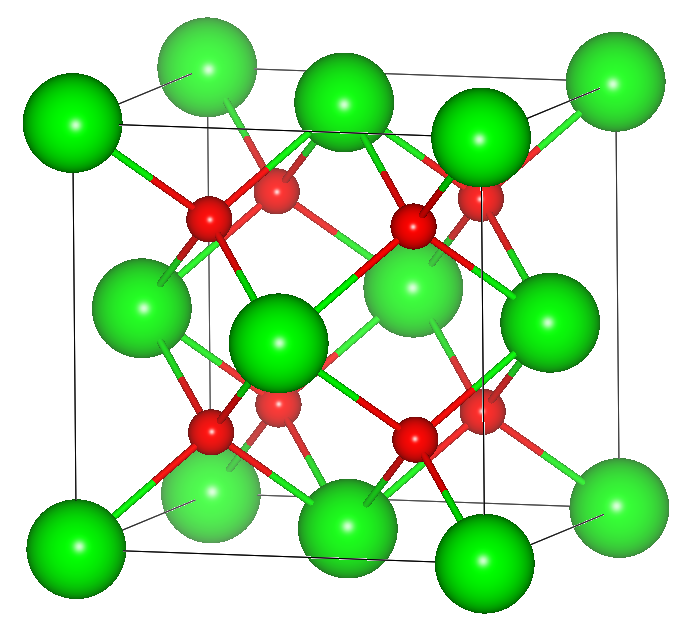
\includegraphics[height=7cm]{images/cubic_unitcell.png}
  \caption{Unit cell of cubic \zirconia . Zirconium atoms are shown in green and oxygen atoms shown in red.}
  \label{fig:cubic_unitcell}
\end{figure}

The lowest specific volume (i.e. highest density) is also exhibited by the cubic phase (11.13 \r{A}$^{3}$ion$^{-1}$) followed by the tetragonal phase (11.51 \r{A}$^{3}$ion$^{-1}$) and then the monoclinic phase (11.99 \r{A}$^{3}$ion$^{-1}$). This is due to it having the largest atomic packing factor, resulting in a mean Zr-O bond distance of 2.22 \r{A}, compared to 2.26 \r{A} in the tetragonal phase and 2.31 \r{A} in the monoclinic phase, as shown in Figure \ref{figure:zrobonddistance}. 

\begin{figure}[h]
\begin{center}
\begin{tikzpicture}
	\begin{axis}
		[width=\linewidth*0.7, xlabel={Nearest neighbour Zr-O bond distance (\r{A})}, ylabel={Relative occurrence}, ymin=0, ymax=140, xmin=2.0, xmax=2.50, legend style={{draw=}, at={(0.95,0.95)}, anchor=north east, legend columns=1}]
		\addplot[no marks] table [x=zr_o_dist, y=monoclinic,]{dat/zr_o_bond_distances.dat}; \addlegendentry{Monoclinic};
        \addplot[no marks, dashed] table [x=zr_o_dist, y=tetragonal, ]{dat/zr_o_bond_distances.dat}; \addlegendentry{Tetragonal};
        \addplot[no marks, densely dotted] table [x=zr_o_dist, y=cubic,]{dat/zr_o_bond_distances.dat}; \addlegendentry{Cubic};
			\end{axis}
		\end{tikzpicture}
		\caption{Density plot of the nearest neighbour Zr-O bond distances in \zirconia\ for each crystal structure. Specific volumes from DFT calculations are 11.99 \r{A}$^{3}$ion$^{-1}$, 11.51 \r{A}$^{3}$ion$^{-1}$, and 11.13 \r{A}$^{3}$ion$^{-1}$ for monoclinic, tetragonal, and cubic phases respectively.}
		\label{figure:zrobonddistance}
	\end{center}
\end{figure}


%\textbf{Also due to the high temperature, the stability of the cubic phase in DFT calculations may be inaccurate. This is discussed further in Chapter 3.}


\subsection{Other phases}

Two orthorhombic phases have also been observed at high pressures in pure \zirconia\ \cite{howard1991crystal}. These structures are referred to as OI and OII, the latter of which is isostructural with cotunnite (PbCl$_{2}$). A third orthorhombic phase ($bc2_{1}$) has also been reported in partially stabilised zirconia (PSZ), but has not been found in pure zirconia \cite{kisi1998crystal}.

\subsubsection{Orthorhombic OI}

The OI phase, illustrated in Figure \ref{fig:orthorhombic_I}, maintains a 7 oxygen coordinated zirconium ion, as is the case in the monoclinic phase. This phase also exhibits two distinct oxygen atom sites like in the monoclinic phase, but being an orthorhombic phase, it does not exhibit a 9\textdegree\ shear in its unit cell like the monoclinic phase. While this phase is briefly stable at high compressive stresses (3.5 - 15 GPa), it appears to be an intermediate phase before collapse into the more familiar cotunnite structure at pressures greater than 15 GPa. In addition, the OI phase is only stable at temperatures below approximately 400 \textdegree C, transitioning to the tetragonal phase at higher temperatures. While PWRs operate at low enough temperatures for the OI phase to be stable, compressive stresses on the order of several GPa will not be present at any significant scale and thus this phase will not affect the oxide microstructure. 


\begin{figure}[htp]
  \centering
      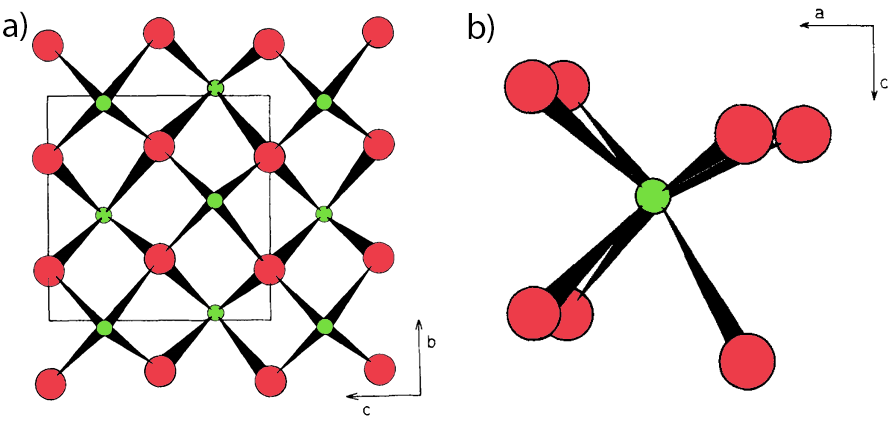
\includegraphics[width=\linewidth]{images/orthorhombic_I.png}
  \caption[Illustrations of the orthorhombic OI (P$bca$) crystal structure of \zirconia\ showing \textbf{a)} the unit cell viewed along the $a$ direction and \textbf{b)} the zirconium ion centre with 7 coordinated oxygen ions. Zirconium and oxygen ions are coloured green and red respectively.]{Illustrations of the orthorhombic OI (P$bca$) crystal structure of \zirconia\ showing \textbf{a)} the unit cell as seen from the $a$ direction and \textbf{b)} the zirconium ion centre with 7 coordinated oxygen ions. Zirconium and oxygen ions are coloured green and red respectively. Adapted from \cite{kisi1989crystal}.}
  \label{fig:orthorhombic_I}
\end{figure}


\subsubsection{Orthorhombic OII (cotunnite)}

The OII phase, illustrated in Figure \ref{fig:cotunnite_structure} maintains a 9 oxygen coordinated zirconium ion. This is due to the high stabilising pressure ($>$ 15 GPa) causing a reduction in the mean interatomic distance, so much so that the zirconium ion, which is typically too small to bond strongly to more than 7 oxygen atoms at standard conditions, can maintain the ninefold oxygen coordination. Such high hydrostatic pressures will not be present in a reactor environment even at the atomic scale, it is therefore not expected to find any OII phase present at any point during the cladding's operational lifetime.

\begin{figure}[htp]
  \centering
      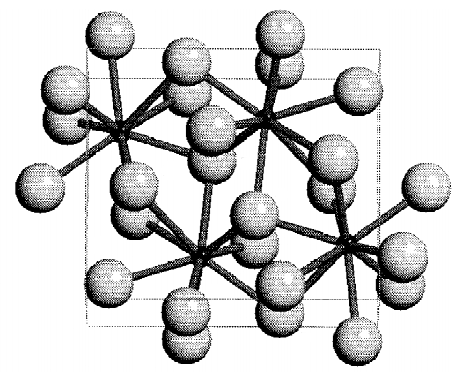
\includegraphics[height=9cm]{images/orthorhombic_II.png}
  \caption[Illustration of the OII cotunnite (P$nma$) crystal structure of \zirconia . Zirconium and oxygen ions are shaded dark and light respectively.]{Illustration of the OII cotunnite (P$nma$) crystal structure of \zirconia . Zirconium and oxygen ions are shaded dark and light respectively. Adapted from \cite{Haines1997}.}
  \label{fig:cotunnite_structure}
\end{figure}

\subsubsection{Hexagonal}

A hexagonal phase of \zirconia\ has also been reported in X-ray diffraction studies at high pressure (20 GPa) and above 1000 \textdegree C \cite{ohtaka1994new}. This phase retains its structure during isobaric quenching, but turns back to monoclinic once pressure is released. This phase is only observed under extreme conditions, and so is mentioned here for purposes of completeness.

%\subsubsection*{Volume expansion}

%The phase transitions in \zirconia\ are accompanied by a change in volume, where the monoclinic phase is the least dense and the cubic phase is the most dense (see Figure \ref{figure:zrobonddistance}). This is especially significant in the case of the martensitic t-\zirconia\ to m-\zirconia\ transition, where the volume increases by around 9\% \cite{Gupta1977}. This has substantial implications for the creation and opening of cracks as \zirconia\ is a ceramic material with low toughness. This is especially relevant in a reactor scenario where temperature cycling (shutdown/startup or load-following behaviour) may lead to fatigue if the phase transition threshold is passed.

%Another consequence of this large volume expansion is that a significant hysteresis effect is observed in the monoclinic/tetragonal phase transition, as shown in Figure \ref{fig:phasediagram}. 
%as the resulting coherency strain is likely to result in reduced mobility of fission products that have been embedded in the bulk crystal. 


\section{Dopant stabilisation}

Particular types of dopants will also stabilise the tetragonal and cubic phases of \zirconia. The most technologically significant is yttrium, which at concentrations of 15\% (atomic), fully stabilises the cubic phase (which in practical terms means the cubic phase is stable down at least to room temperature). Zirconia stabilised this way is known as yttria-stabilised zirconia (YSZ). The inclusion of trivalent yttrium promotes the inclusion of charge compensating oxygen vacancy defects (see Equation \ref{equation:YSZ} which uses Kr\"{o}ger-Vink notation, explained in the next section). This works in a similar way with several other cation dopants such as trivalent scandium from Sc$_{2}$O$_{3}$, or divalent magnesium from MgO (Equation \ref{equation:mg_stabilised_zro2}), which also act as cubic stabilisers.

{\setstretch{1.5}
\begin{equation}
\ch{Y_{2}O_{3}} = 2\ch{Y_{Zr}^{'}} + \ch{V_{O}^{**}} + 3\ch{O_{O}^{x}} 
\label{equation:YSZ}
\end{equation}

\begin{equation}
\ch{MgO} = \ch{Mg_{Zr}^{''}} + \ch{V_{O}^{**}} + \ch{O_{O}^{x}} 
\label{equation:mg_stabilised_zro2}
\end{equation}
}

As already discussed above, while MO$_{2}$ oxides (e.g. CeO$_{2}$) often adopt the regular cubic fluorite structure, we only observe cubic stabilisation  of \zirconia\ at elevated temperatures where the effective ionic radii of the zirconium ion increases (possibly due to a stabilising phonon mode contribution). Yttrium stabilises the cubic phase because the yttrium ion is of the appropriate size to maintain its surrounding oxygen ions (which may include a vacant oxygen site) in the VIII coordination at low temperatures. This is supported by the ionic radii values in Table \ref{figure:ionicradii} which shows that the Y$^{3+}$ radii are even larger than the Ce$^{4+}$ radii and clearly larger than the corresponding Zr$^{4+}$ radii. 

%This is accomplished by substituting a Zr\textsuperscript{4+} ion with Y\textsuperscript{3+} and the binding of two neighbouring oxygen vacancies, effectively producing a sub-unit of yttria (Y\textsubscript{2}O\textsubscript{3}) in the \zirconia\ lattice. 

\begin{table}[htp]
\onehalfspacing
\centering
\caption[Ionic radii of Zr$^{4+}$, Y$^{3+}$ and Ce$^{4+}$ in various coordination environments.]{Ionic radii of Zr$^{4+}$, Y$^{3+}$ and Ce$^{4+}$ in various coordination environments. Values taken from \cite{Shannon1976}.}
\label{figure:ionicradii}
\begin{tabular}{ccc}
\hline
Ion & Coordination & Ionic Radius (\r{A}) \\ \hline
\multicolumn{1}{c}{\multirow{6}{*}{Zr$^{4+}$}} & \multicolumn{1}{c}{IV} & 0.59 \\
\multicolumn{1}{c}{} & \multicolumn{1}{c}{V} & 0.66 \\
\multicolumn{1}{c}{} & \multicolumn{1}{c}{VI} & 0.72 \\
\multicolumn{1}{c}{} & \multicolumn{1}{c}{VII} & 0.78 \\
\multicolumn{1}{c}{} & \multicolumn{1}{c}{VIII} & 0.84 \\
\multicolumn{1}{c}{} & \multicolumn{1}{c}{IX} & 0.89 \\ \hline
\multicolumn{1}{c}{\multirow{4}{*}{Y$^{3+}$}} & \multicolumn{1}{c}{VI} & 0.90 \\
\multicolumn{1}{c}{} & \multicolumn{1}{c}{VII} & 0.96 \\
\multicolumn{1}{c}{} & \multicolumn{1}{c}{VIII} & 1.019 \\
\multicolumn{1}{c}{} & \multicolumn{1}{c}{IX} & 1.075 \\ \hline
\multicolumn{1}{c}{\multirow{4}{*}{Ce$^{4+}$}} & \multicolumn{1}{c}{VI} & 0.87 \\
\multicolumn{1}{c}{} & \multicolumn{1}{c}{VIII} & 0.97 \\
\multicolumn{1}{c}{} & \multicolumn{1}{c}{X} & 1.07 \\
\multicolumn{1}{c}{} & \multicolumn{1}{c}{XII} & 1.14 \\
\end{tabular}
\end{table}

\section{Kr\"{o}ger-Vink notation}

Kr\"{o}ger-Vink notation \cite{kroger1956relations} is used throughout this thesis to describe defects. It is widely used in physical chemistry and is a useful shorthand for describing chemical reactions where conservation of mass, charge and lattice sites is required. The notation syntax is of the form \ch{x^{y}_{z}}, where x is the substituted atom or missing atom (i.e. a vacancy V), y is the charge of the defect (relative to the lattice species that originally occupied the site) and z is the site the defect occupies. Positive and negative charges are indicated with dots (\ch{^{*}}) and dashes (\ch{^{'}}) respectively, otherwise a cross (\ch{^{x}}) is used to denote a neutral defect. The site may be either a lattice site (such as Zr or O in \zirconia ) or an interstitial site ($i$). Table \ref{table:krogervink} shows examples of several different types of defects and their respective Kr\"{o}ger-Vink notation.

\begin{table}[htp] % Kroger-Vink notation table
\onehalfspacing
\centering
\caption{Examples of Kr\"{o}ger-Vink notation for several defects in \zirconia .}
\label{table:krogervink}
\begin{tabular}{cc}
\hline
Defect & Kr\"{o}ger-Vink Notation \\ \hline
Anion vacancy & \ch{V_{O}^{**}} \\
Cation vacancy & \ch{V_{Zr}^{''''}} \\
Anion interstitial & \ch{O_{i}^{''}} \\
Cation interstitial & \ch{Zr_{i}^{****}} \\
Iodine (I$^{-}$ anion) on oxygen site & \ch{I_{O}^{*}} \\
Iodine (I$^{+}$ cation) on zirconium site & \ch{I_{Zr}^{'''}} \\ \hline
\end{tabular}
\end{table}

